\section{Zielsetzung}
\label{sec:Zielsetzung}

Ziel des Versuches ist es das Anregungs- und Dämpfungsverhalten eines LRC-Schwingkreises
bei Wechselstrom verschiedener Frequenzen zu beschreiben.


\section{Theorie}
\label{sec:Theorie}

\subsection{Dämpfung des Stroms in einem Schwingkreis}

Zunächst wird der folgende Schwingkreis betrachtet, welcher durch einen
kurzen Strompuls in Gang gesetzt wird und danach abklingt.

\begin{figure}[H]
  \centering
  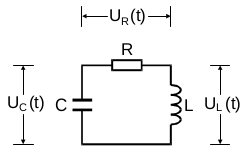
\includegraphics{content/images/V354.png}
  \caption{Gedämpfter L-R-C-Schwingkreis.}
  \label{fig:schwingkreis}
\end{figure}

Für den Stromkreis in Abbildung \ref{fig:schwingkreis} gilt die
DGL:
\begin{equation}
  U_C(t)+U_R(t)+U_L(t)=0
\end{equation}
Für den beschriebenen Strompuls kann die Lösung der DGL mathematisch durch die Überlagerung einer
einhüllenden Funktion und einer sinus/cosinus Funktion dargestellt werden.

\begin{figure}[H]
  \centering
  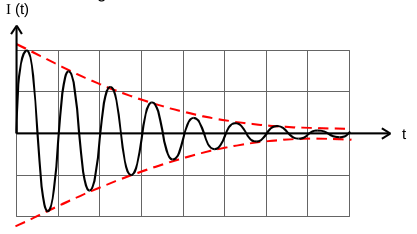
\includegraphics{content/images/dia.png}
  \caption{Dämpfungskurve des Stroms.}
  \label{fig:daempfung}
\end{figure}


\begin{align}
  \symbf{I} &= I_0 e^{-2\pi\mu t}
  \cdot\text{cos}\left(2\pi\nu t+\eta\right)\\
  \symbf{I}_\text{einhüllend} &= I_0 e^{-2\pi\mu t}
  \label{eqn:einhuellend}
\end{align}

\subsection{Grenzwiderstand für den aperiodischen Grenzfall}

\begin{figure}[H]
  \centering
  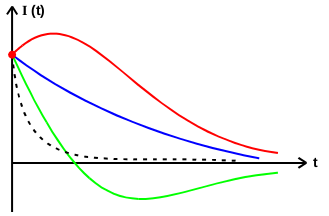
\includegraphics{content/images/dia2.png}
  \caption{Dämpfungskurve des Stroms.}
  \label{fig:aperiodisch}
\end{figure}

Nach der Bestimmung des Dämpfungsverhaltens eines Schwingkreises
wird nun der Widerstand $R_\text{ap}$ berechnet für welchen der
Strom im Schwingkreis am schnellsten gegen null läuft. Dieses
Phänomen wird aperiodischer Grenzfall genannt und wird durch
die gestrichelte Linie in Abbildung \ref{fig:aperiodisch}
dargestellt. Ist der Widerstand zu hoch, so wirkt die Gegeninduktion der
Spule verlangsament und der Graph fällt wie wie der rote oder der
blaue Graph in Abbildung \ref{fig:aperiodisch}, ist er zu hoch
ergibt sich einen Überschwingen wie beim grünen Graphen.
Mathematisch lässt sich dies über die Periodendauer T des
Schwingkreises bestimmen.
\begin{equation}
  T = \frac{2\pi}{\sqrt{1/LC-R^2/4L^2}}
\end{equation}
Der Grenzfall tritt für $T\to\infty$ auf:
\begin{align}
  \implies \frac{1}{LC}&=\frac{R_\text{ap}^2}{4L^2}\\
  \iff R_\text{ap} &=\sqrt{\frac{4L}{C}}
\end{align}
